\documentclass[assignment07_Solutions]{subfiles}

\invalidatemargin

\IfSubStr{\jobname}{\detokenize{Solutions}}{\toggletrue{solutions}}{\toggletrue{solutions}}

%\IfSubStr{\jobname}{\detokenize{Solutions}}{\toggletrue{solutions}}{\togglefalse{solutions}}

\fancypagestyle{firstpage}

{\rhead{Assignment 7 \linebreak \textit{Version: \today}}}

\title{Assignment 7: Pytorch, Vanishing Gradients, and Convolutional Neural Networks}
\author{Machine Learning}
\date{Fall 2019}

\begin{document}

\maketitle
\thispagestyle{firstpage}


\begin{learningobjectives}
\bi
\item Learn the basics of Pytorch
\item Understand the vanishing gradient problem and how to fix it
\item Learn about convolutional neural networks from a conceptual perspective
\item Apply convolutional neural networks to a real dataset.
\ei
\end{learningobjectives}

\begin{priorknowledge}
\bi
\item Multilayer perceptron
\item Backpropagation
\ei
\end{priorknowledge}

\section{Pytorch and Autograd Algorithms}
TODO Pytorch tutorial

\section{Backpropagation and the Problem of Vanishing (or Exploding) Gradients}

\begin{recall}[Multi-layer perceptron]
The multi-layer perceptron consists of a bunch of single-layer perceptrons stacked on top of each other.  Last assignment we saw a particular special case of this where we just a few logistic regression models and stack them.  A cartoon version of the network applied to the titanic dataset is shown below.

\begin{center}
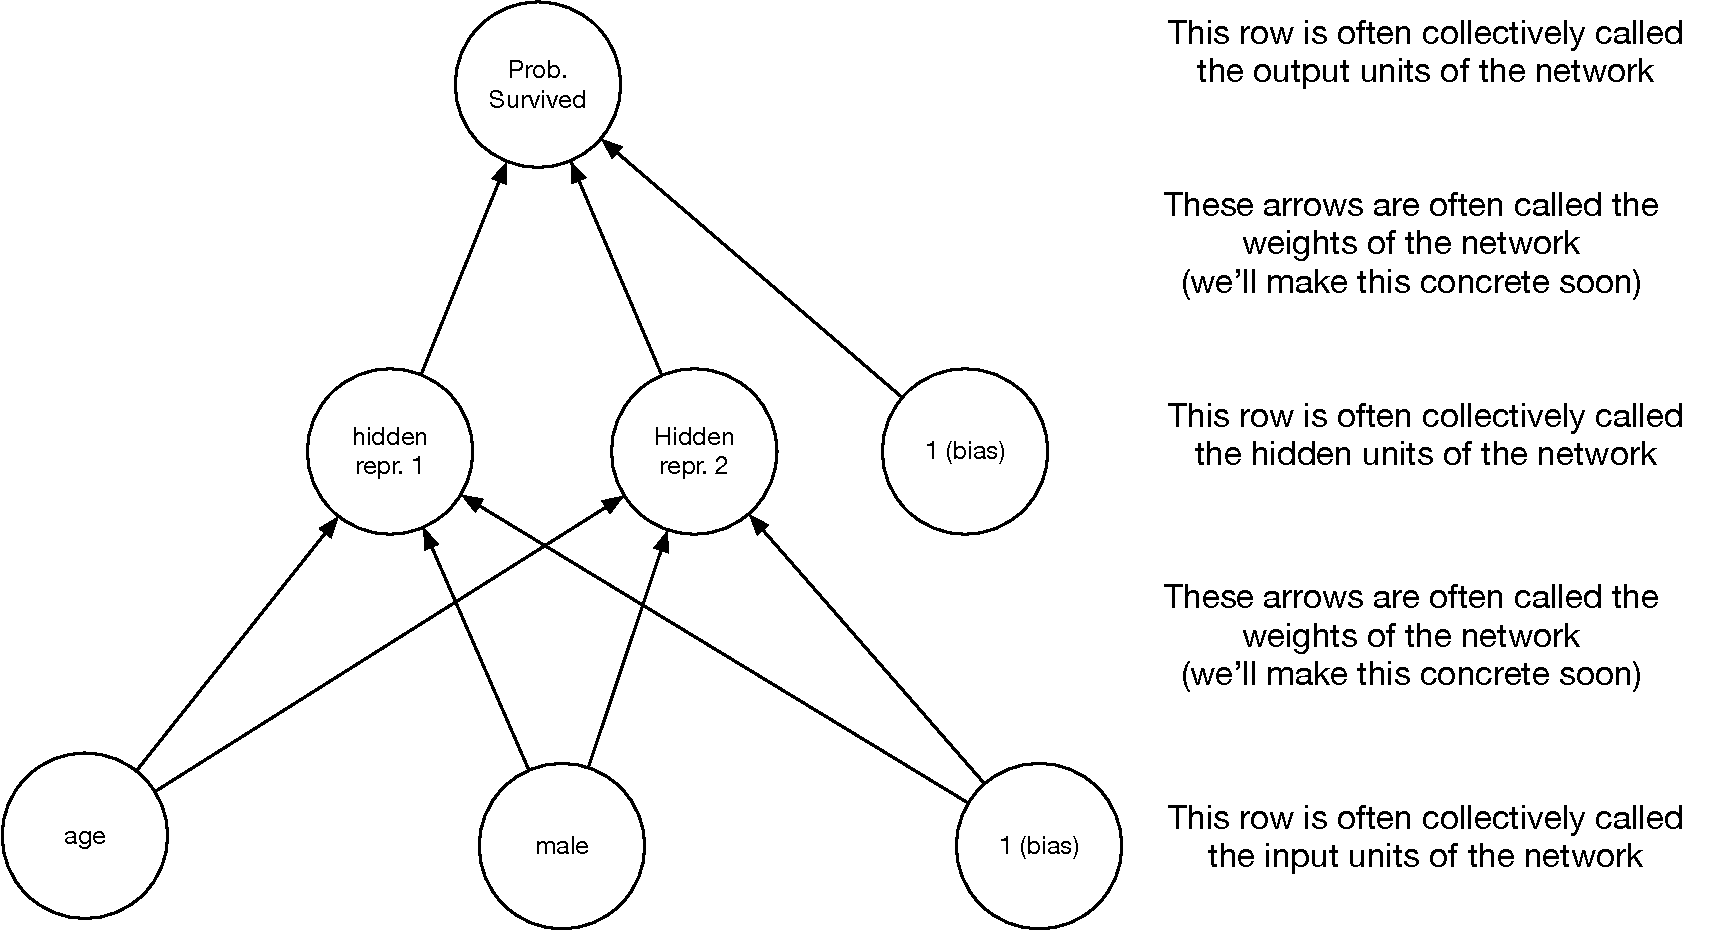
\includegraphics[width=0.7\linewidth]{figures/titanicmlpsimple}
\end{center}

We saw in the companion notebook that the network that networks of this type are capable of.  We can make things even more precise by zooming in on how data propagates from lower layers to higher layers (view 1 in the figure below) and ultimately to the loss function (view 2 the figure below), which helps us understand how to tune our weights to the data.

\vspace{1em}

Notation Guide:
\vspace{1em}

\begin{tabular}{| c | l |}
\hline
$l$ & the loss function for the network (log loss in this case) \\
\hline
$m$ & the number of layers in the network \\
\hline
$n_{k}$ & the number of nodes in the $k$th layer \\
\hline
$x_j^{(k)}$& The $j$th node in the $k$th layer of the network ($k = 1$ is the input \\
&and $k = m$ is the output) \\
\hline
$\mathbf{x^{(k)}}$ & The nodes at the $k$th layer in vector form \\
\hline
$s_{i}^{(k)}$ & the $i$th summation node in the $k$th layer \\
\hline
$w_{i,j}^{(k)}$ & the weight connecting the $j$th node in layer k to the $i$th node in\\
&  layer $k+1$ \\
\hline
$\mlvec{w_{i}^{(k)}}$ & the vector of weights to the $i$th summation node in layer $k+1$.\\
\hline
\end{tabular}

\begin{center}
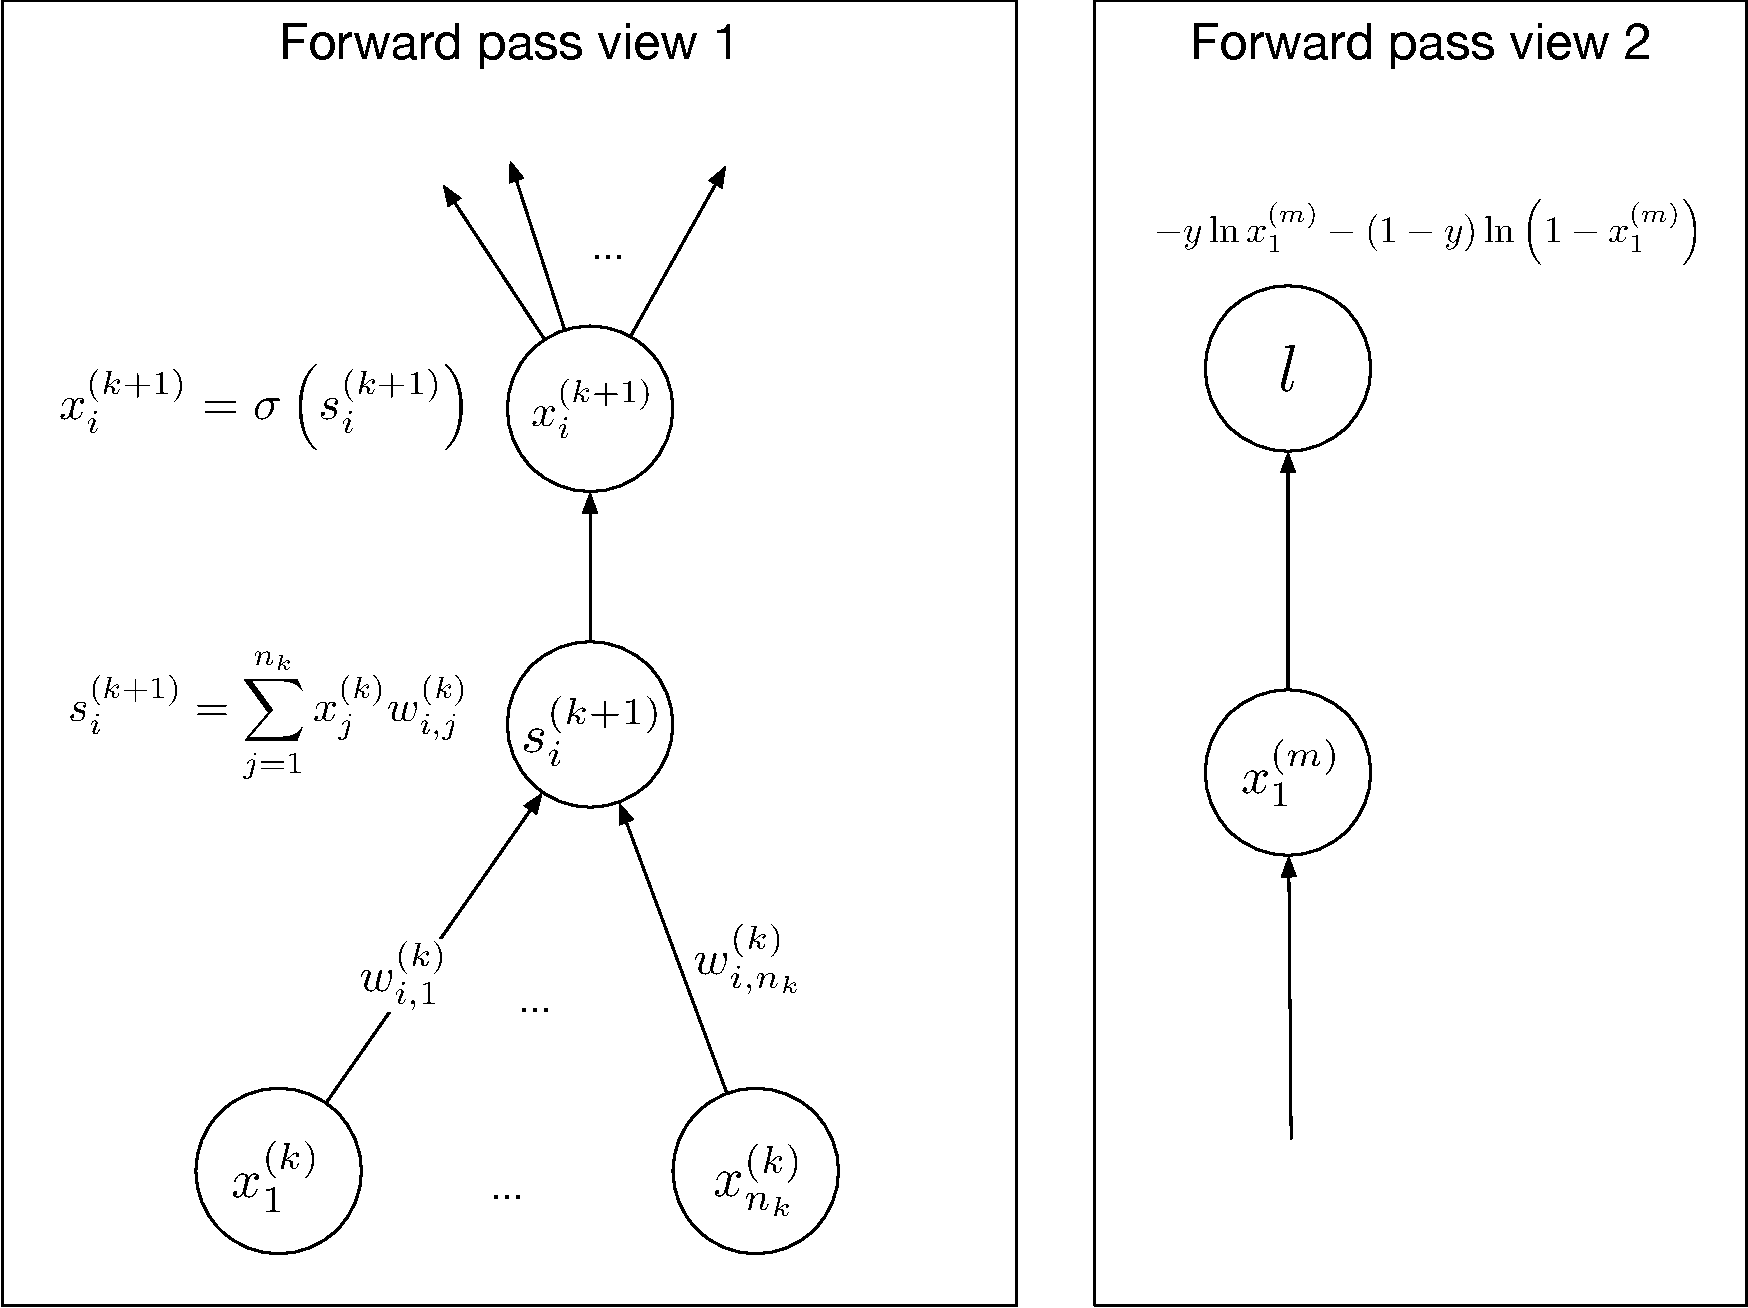
\includegraphics[width=0.7\linewidth]{figures/mlpfullforward}
\end{center}

\end{recall}

In the previous assignment you derived the backpropagation algorithm, which can be used to compute the gradient of the weights in an MLP with respect to the loss function.  What's beautiful about this formula is that it works for networks of arbitrary depth.  You may have heard of \href{https://en.wikipedia.org/wiki/Deep_learning}{deep learning}, which is where networks of dozens or even hundreds of layers are trained on a particular task.  Despite their complexity, these networks are typically trained using the backpropagation algorithm you met in the last assignment!

Despite the relative simplicity of the backpropagation equations, there are some dangers lurking when applying the algorithm to deep networks ($m$ very large).  The most common pitfalls that one encounters are \textbf{vanishing and exploding gradients}.  A vanishing gradient is when the gradient of the loss with respect to the weights in a layer becomes vanishingly small as you move from the output layer back towards the input layer.  An exploding gradient is the opposite problem (when the gradient of the loss with respect to the weights in a layer becomes exceedingly large as you move from the output layer towards the input layer).

\begin{exercise}[(30-90 minutes)]
Before starting this exercise, go and learn about the vanishing gradient problem.  Here are a few resources to look at.  You do not need to read all of them, so please pick the ones that seem the most inline with how you learn.
\begin{externalresources}
\bi
\item \href{https://ayearofai.com/rohan-4-the-vanishing-gradient-problem-ec68f76ffb9b}{Rohan Kapur's Intuitive Explanation of the Vanishing Gradient Problem}
\item \href{https://www.youtube.com/watch?v=SKMpmAOUa2Q}{Deep Learning Simplified: An Old Problem}
\item \href{https://en.wikipedia.org/wiki/Vanishing_gradient_problem}{Vanishing Gradient Problem on Wikipedia} (we recommend you stop reading once you get to the section marked \emph{Solutions}.
\ei
\end{externalresources}


Last assignment we derived the following backpropagation equations.

\begin{align}
(\nabla_{\mathbf{w^{(k)}_i}}) l &= \mlvec{x^{(k)}} \sigma\left (s_i^{(k+1)} \right )\left (1-\sigma\left (s_i^{(k+1)} \right )\right) \frac{\partial l}{\partial x_i^{(k+1)}} \\
\frac{\partial l}{\partial x^{(k)}_i} &= \sum_{j=1}^{n_{k+1}} w^{(k)}_{j,i} \sigma \left ( s_{j}^{k+1} \right) \left (1-\sigma \left ( s_{j}^{k+1} \right)\right) \frac{\partial l}{\partial x^{(k+1)}_j} \label{eq:recursion} \\
\frac{\partial l}{\partial x^{(m)}_1} &= -y\frac{1}{x_1^{m}} + (1-y) \frac{1}{1-x_1^{(m)}} 
\end{align}

\bes
\item If we examine these equations, we can understand much better where the vanishing gradient problem comes from.  In particular, Equation~\ref{eq:recursion} provides the crucial recursive formula for defining the partial derivatives of the loss with respect to nodes in the network in terms of the same partial derivatives for nodes deeper in the network (i.e., closer to the output).  Based on Equation~\ref{eq:recursion}, what aspects of the network might contribute to or counteract the vanishing gradient problem.  Consider things such as the values of the summation units $s_j^{(k+1)}$, the values of the weights, and the number of units eat each layer of the network ($n_k$).
\item It turns out that the use of the sigmoid function to transform the summation units when calculating the values at the next layer is not the only viable choice. It turns out that many different types of non-linear functions can be used (e.g., \href{http://mathworld.wolfram.com/HyperbolicTangent.html}{tanh}).  The function used in this capacity is called an \emph{activation function}.  If we let $a$ refer to our activation function, then Equation~\ref{eq:recursion} becomes

\begin{align}
\frac{\partial l}{\partial x^{(k)}_i} &= \sum_{j=1}^{n_{k+1}} w^{(k)}_{j,i} a' \left ( s_{j}^{k+1} \right)  \frac{\partial l}{\partial x^{(k+1)}_j} \label{eq:recursion2} \enspace .
\end{align}


One very popular choice of activation function is called \href{https://en.wikipedia.org/wiki/Rectifier_(neural_networks)}{rectified linear} (or ReLu for \emph{rectified linear unit}).  A graph of the ReLu activation function is shown below.

\begin{center}
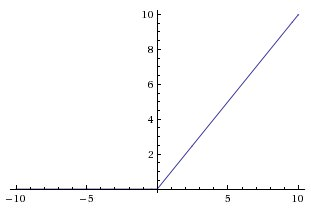
\includegraphics[width=0.4\linewidth]{figures/relu}
\end{center}

How does choosing the ReLu as an activation function help with the vanishing gradient problem versus choosing the sigmoid.

\item \textbf{Going Beyond (optional)} Using pytorch, perform a computational investigation of the vanishing gradient problem.  We suggest the following steps (note: we have our own version of this in the solutions file if you want to check it out):
\bi
\item Create an MLP where the number of layers is passed in as a parameter.
\item Before doing any training of the network, feed an arbitrary input into the network, compute the loss, and then compute the gradient of the loss with respect to the weights at each level of the network.
\item Summarize the partial derivatives of the weights at each level in the network (e.g., take the mean of the absolute values) and plot this quantity as a function of $k$ (the layer number).  It may be helpful to use a log scale for the y-axis.
\ei
\ees

\end{exercise}

\section{Convolutions and Image Filtering}

Depending on your math background you may have seen the convolution operation before.

\begin{externalresources}[(30 minutes)]
\bi
\item \href{http://machinelearninguru.com/computer_vision/basics/convolution/image_convolution_1.html}{Image Filtering}
\item Video: \href{https://www.youtube.com/watch?v=C_zFhWdM4ic}{How blurs and filters work}
\ei
\end{externalresources}

\section{Convolutional Neural Networks}
Quick blurb here.
\begin{externalresources}[(60 minutes)]
\bi
\item \href{https://ujjwalkarn.me/2016/08/11/intuitive-explanation-convnets/}{Intuitive Explanation of Convnets}
\item \href{http://scs.ryerson.ca/~aharley/vis/conv/flat.html}{Beautiful interactive visualization of a Convnet trained to recognize handwritten digits} (don't miss this one!)
\item \href{https://www.datascience.com/blog/convolutional-neural-network}{Convolutional Neural Networks Explained}
\item \href{https://www.youtube.com/watch?v=bNb2fEVKeEo&list=PL3FW7Lu3i5JvHM8ljYj-zLfQRF3EO8sYv\&index=5}{Lecture 5 from CS231 at Stanford} (it starts getting a bit too low-level around the 35 minute mark)
\ei
\end{externalresources}

\section{Training Your First Convnet}

TODO: NINJAs to work on this.

\section{Something on Context and Ethics and Convnets (if we pushed project out another day, I would vote for this}

\section{Getting Ready for the Project}
Sam to work on this.
\subsection{Goals}
\subsection{Datasets}

\end{document}
